%!TEX root = ../main.tex
\chapter{Android Reverse Engineering}
Java is the basis of Android applications and has historically been what is used. Java is particularly well-suited for reverse engineering due to its architecture. It is designed to be platform-independent by running on the Java Virtual Machine (JVM), which functions as an abstract computing environment with its own instruction set and memory model. The JVM interprets a binary format known as a class file, which contains bytecode (JVM instructions), a symbol table, and metadata.

The JVM is stack-oriented, with most operations involving the operand stack in the current execution frame. New frames are created whenever methods are invoked, providing a clear and modular structure. This design simplifies the decompilation and analysis process, which is critical when reconstructing application logic and behavior ~\cite{jvms8}.
Figure\ref{fig:javaprocess} illustrates the flow of data from Java source code through compilation, class loading, bytecode verification, and execution by the JVM.
\begin{figure}
	\centering
	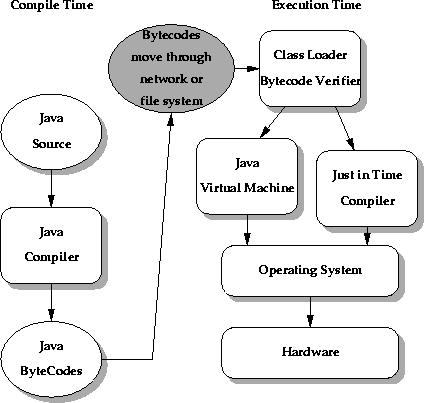
\includegraphics[scale=.7]{java_process.png}
	\caption{Java Source to Hardware}
	\label{fig:javaprocess}
\end{figure}

The use of class files is one of the key factors that makes reverse engineering Java-based applications more straightforward. Unlike many other languages that are compiled directly into low-level assembly, Java is compiled into bytecode, an intermediate representation that retains a significant amount of the original structure of the source code. This structure provides helpful context for decompilation tools.
As noted by Alex Kalinovsky, “bytecode can be interpreted or compiled after loading, which results in a two-step transformation of the high-level programming language into the low-level machine code. It is the intermediate step that makes decompiling Java bytecode nearly flawless" \cite{covertjava}. Bytecode preserves nearly all critical information from the source file, with the exception of comments and formatting. Method names, variables, and control flow are typically intact, making it easier to reconstruct the original logic. Additionally, the stack-oriented design the JVM offers a predictable execution model that further aids analysis.

A man-in-the-middle (MITM) approach utilizing instrumentation was selected for its relative simplicity compared to full decompilation or bytecode-level modification. In this context, the MITM or instrumentation method refers specifically to intercepting communication between the client application and the device it controls (e.g., a host device such as a Bluetooth-connected peripheral). This strategy includes techniques such as using Bluetooth sniffers to capture transmitted data and injecting code at runtime to observe or alter behavior without directly modifying the underlying APK or its bytecode.


\section {A Brief Overview of Android Fundamentals}
To understand the reverse engineering process of an Android application, it’s helpful to start with some foundational knowledge. At the most basic level, an Android app is made up of activities and layouts. Activities are special classes, typically written in Kotlin, that control how the app behaves and responds to user input. For example, if an app has a button, the activity defines what happens when that button is clicked. 

Most Android apps have one or more screens, and the design of these screens is handled through layout files or directly in the activity code. Layout files are usually written in XML and can include elements like text, images, and buttons ~\cite{headfirstandroid}. Figure \ref{fig:activitylayout} shows a diagram of activities and layouts. Figure \ref{fig:activitylayoutprocess} illustrates how they interact during actual device use.
\begin{figure}[H]
	\centering
	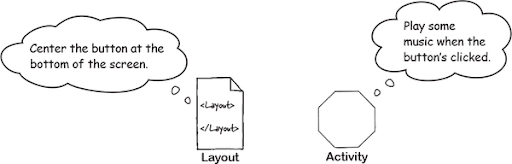
\includegraphics[scale=0.65]{activity_layout.png}
	\caption{Android Activity Layout}
	\label{fig:activitylayout}
\end{figure}
\begin{figure}[H]
	\centering
	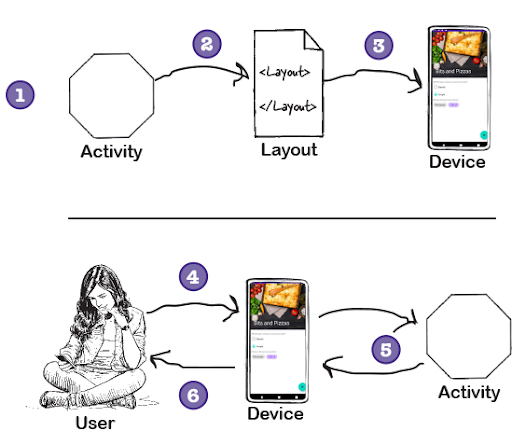
\includegraphics[scale=0.35]{activity_layout_process}
	\caption{Android Activity to User}
	\label{fig:activitylayoutprocess}
\end{figure}

\begin{itemize} 
	\item Android launches the app’s main activity.
	\item The activity instructs Android to use a specific layout.
	\item The layout is displayed on the device.
	\item The user interacts with the layout.
	\item The activity responds to these interactions and updates the display.
	\item The user is able to view the updated display seamlessly.
\end{itemize}

Apps are built using the Android Software Development Kit. The most straightforward place to do this is the Android Studio app. The Android SDK has Android source files and a compiler used to compile code into the Android format.

% TODO: \usepackage{graphicx} required
\begin{figure}[H]
	\centering
	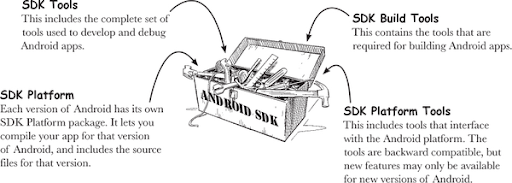
\includegraphics[width=0.7\linewidth]{android_sdk_tools.png}
	\caption{Androiod SDK Tools}
	\label{fig:androidsdktools}
\end{figure}

If you’re familiar with Android, you’ve probably encountered its fun, food-based versioning system. Each Android version includes a version number and a code name. The version number refers to the specific release (like 8.0), while the code name represents a broader release range (like Oreo). Google stopped using dessert-themed code names after Android 9. Each version of Android also corresponds to an API level, which is used by apps to ensure compatibility. For example, Android 11 corresponds to API level 30. Android Studio projects use the Gradle build system to compile and deploy apps. Gradle-based projects follow a standard directory structure, which is shown in Figure \ref{fig:gradlebuildstructure}.

% TODO: \usepackage{graphicx} required
\begin{figure}[H]
	\centering
	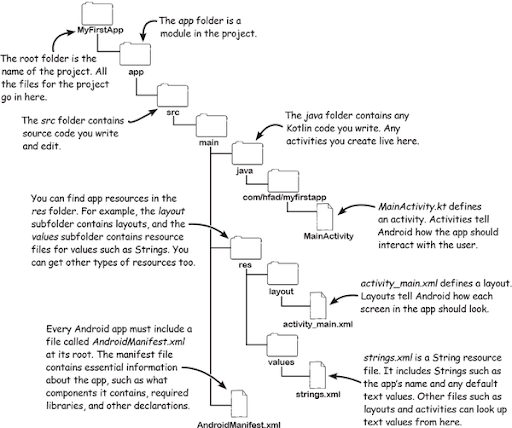
\includegraphics[width=0.7\linewidth]{gradle_build_structure.png}
	\caption{Gradle Build Structure}
	\label{fig:gradlebuildstructure}
\end{figure}
A much larger version of this structure is seen in the decompilation of the Persolips app. 

An Android app is made up of four main components: activities, services, broadcast receivers, and content providers. Each of these acts as an entry point into the app, either for the user or the system. Some components operate independently, while others rely on or interact with each other. As mentioned before, Activities are the entry points that users interact with directly. Each activity represents a single screen with a user interface. In a note-taking app, for example, you might have one activity for composing a note, another for creating folders, and another for reading existing notes. While each activity functions independently, they work together to provide a cohesive user experience. Activities can even be started by other apps—if permissions allow. For instance, the Photos app might open a note composition activity so an image can be saved directly into a note.

Activities also manage key interactions between the system and the app. They help Android determine what’s important to the user and ensure that relevant processes are kept running. They track backgrounded processes that might be reopened and help manage killed processes so their state can be restored if needed. Activities enable apps to work together and let the system coordinate those interactions. In code, activities are implemented as subclasses of Android’s Activity class.

Services are also entry points, but they run in the background and are designed for general-purpose tasks rather than direct user interaction. They’re used to keep apps running behind the scenes—for example, to perform long-running operations or interact with remote processes. A service has no user interface. It might do something like keep the flashlight on while a user switches to another app or fetch data from the internet without interrupting the user’s experience. Activities and other components can start services and allow them to run independently or bind to them.

There are two types of services: started services and bound services. A started service continues to run even if the user leaves the app—like keeping the flashlight on or syncing data in the background. Services that the user is aware of (like the flashlight) are handled differently than those that operate silently (like data syncing). Bound services, on the other hand, only run when another component is actively connected to them.

Broadcast receivers allow the system to deliver messages or events to apps, even if the app isn't currently running. This makes it possible to respond to system-wide events outside of the usual user flow. For example, a scheduled notification could be delivered through a broadcast receiver without needing the app to stay open.
Content providers manage access to data stored outside of the app itself, such as in a local SQLite database, on the device, or in the cloud. They make it possible for apps to query or modify this data securely. For example, a social networking app might use a content provider to access the user’s device contacts when adding new friends.

When an Android app is packaged and deployed, it’s bundled into a file called an APK (Android Package Kit). This file contains everything needed to install and run the app on a device. Figure \ref{fig:apktoapp} outlines the typical structure of an APK.
Kotlin source code is compiled into bytecode, and libraries and resources are gathered. These elements are then assembled into the APK. The contents of an APK typically include:
\subsection{Structure of an APK File}

An APK file is a ZIP archive typically containing:

\begin{itemize}
  \item \textbf{META-INF/}: Contains cryptographic metadata.
  \begin{itemize}
    \item \texttt{MANIFEST.MF}: Lists files with SHA-1 digests.
    \item \texttt{CERT.SF}, certificate files: Signatures ensuring integrity.
  \end{itemize}
  \item \textbf{lib/}: Native libraries compiled per architecture (e.g., \texttt{armeabi-v7a}, \texttt{arm64-v8a}, \texttt{x86}, \texttt{x86\_64}).
  \item \textbf{res/}: Application resources (images, layouts), not compiled into \texttt{resources.arsc}.
  \item \textbf{assets/}: Raw asset files accessible via \texttt{AssetManager}.
  \item \textbf{AndroidManifest.xml}: App metadata in binary XML (can be decoded using tools like Apktool or Androguard).
  \item \textbf{classes.dex}: Bytecode in Dalvik Executable (DEX) format for the Android Runtime.
  \item \textbf{resources.arsc}: Precompiled binary resources (e.g., strings, styles).
\end{itemize}

All of these components work together to form the complete, installable app package. When installed, the Android system unpacks the APK and sets up everything the app needs to run on the device.
% TODO: \usepackage{graphicx} required
\begin{figure}[H]
	\centering
	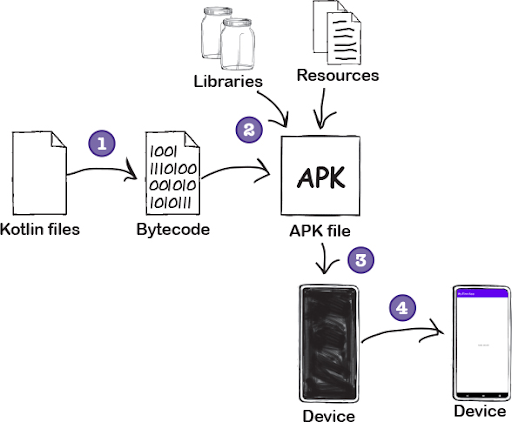
\includegraphics[scale=.65]{apk_to_app.png}
	\caption{Android App Components}
	\label{fig:apktoapp}
\end{figure}

\section[Overview of the YSL Makeup Printer]{Overview of the Yves Saint Laurent Makeup Printer (Rouge Sur Mesure Custom Lip Color Creator)}
One of the most basic yet crucial steps in reverse engineering a device is acquiring a comprehensive understanding of its functionality. The YSL makeup printer is a unique device, and it is therefore essential to examine its components in order to contextualize any observed or modified behavior.

At its core, the device functions as a lipstick dispenser capable of mixing precise quantities of pigment to produce custom colors. It operates in tandem with the Rouge Sur Mesure application. Within the app, users can select colors in one of three ways: shade matching from photographs, choosing from a color wheel, or employing YSL’s shade stylist, which uses outfit analysis to recommend a complementary lip color. When executing a dispense cycle, the interface progresses through three primary screens. Initially, it displays the selected shade, followed by a progress screen featuring three dots and the label of the inserted color family, and finally the device presents the successfully printed color. According to YSL, “Rouge Sur Mesure uses custom color cartridges and artificial intelligence to make and recommend over 7,000 unique lip colors” \footnote{ https://www.yslbeautyus.com/rouge-sur-mesure.html?srsltid=AfmBOorRGtCnqu9Hg\_-\_9mebHE1hqicByITz-JtpICKBy8BZVciVP-ml }. The system leverages PERSO technology, L’Oréal’s latest innovation in personalized beauty, to analyze user data and tailor product recommendations to each individual. Figure \ref{fig:makeupprinter} presents an image of the device, Figure \ref{fig:colorwheel} illustrates the color wheel selection interface, and Figure \ref{fig:colorselector} shows the image-based shade matching screen.
% TODO: \usepackage{graphicx} required
\begin{figure}[H]
	\centering
	
\includegraphics[scale=1.1]{makeupprinter}
	\caption{Rouge Sur Mesure Custom Lip Color Creator}
	\label{fig:makeupprinter}
\end{figure}

% TODO: \usepackage{graphicx} required
\begin{figure}[H]
	\centering
	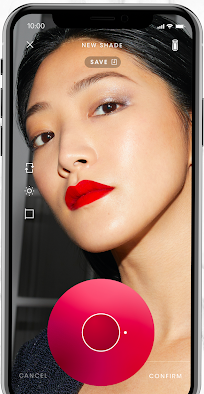
\includegraphics[scale=.7]{colorwheel}
	\caption{Color Wheel App Screen}
	\label{fig:colorwheel}
\end{figure}

% TODO: \usepackage{graphicx} required
\begin{figure}[H]
	\centering
	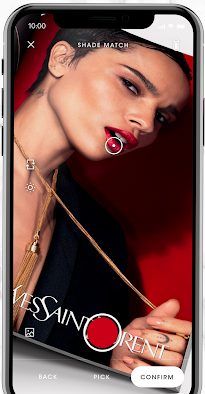
\includegraphics[scale=.7=]{colorselector}
	\caption{Color from Image App Screen}
	\label{fig:colorselector}
\end{figure}

Despite the promise of limitless customization, the device’s actual capabilities are more constrained. It contains three slots into which cartridges from one of seven color families: red, nude, orange, pink, warm red, warm nude, and cool nude may be inserted. Figure \ref{fig:colorfamilies} displays the color wheel grouped by family, and Figure \ref{fig:cartridges} depicts the physical cartridges, including the cool nude sample used in this analysis. Each color family must be purchased separately, and at the time of writing, the cost per family is approximately \$65 USD.

% TODO: \usepackage{graphicx} required
\begin{figure}[H]
	\centering
	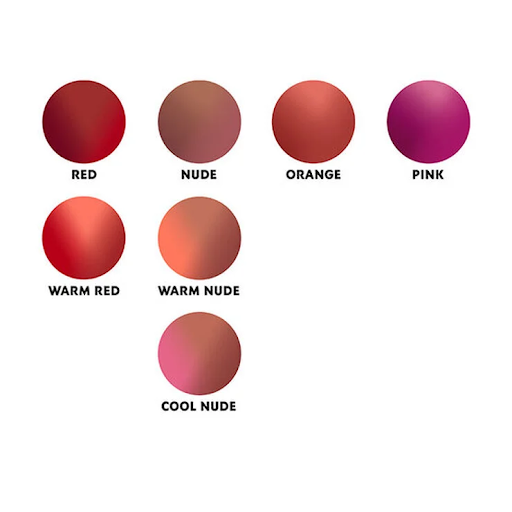
\includegraphics[scale=.5]{colorfamilies}
	\caption{Rouge Sur Mesure Color Families}
	\label{fig:colorfamilies}
\end{figure}

% TODO: \usepackage{graphicx} required
\begin{figure}[H]
	\centering
	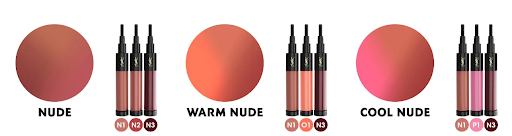
\includegraphics[scale=.5]{cartridges}
	\caption{Rouge Sur Mesure Cartridge Trios}
	\label{fig:cartridges}
\end{figure}


These limitations reveal that the system does not fully eliminate the need for multiple lipstick purchases. Although the app can generate custom shades within a single color family, the presence of three distinct "nude" families underscores that users must still invest in multiple cartridges to achieve a broad spectrum of tones. Additionally, many users report that the printer struggles to reproduce an exact match for the selected custom color. In my own testing, the device seldom produces an exact duplicate of the chosen shade; instead, it defaults to the closest available hue within the loaded family. To encourage additional purchases, the application will notify users if a slightly closer match exists in an unloaded color family, prompting them to acquire that family.

Understanding the functionality of the device overall is essential for correlating the data captured during reverse engineering with its operational components.

\section{Reverse Engineering the Rouge Sur Mesure App}

Makeup enthusiasts are all too familiar with the struggle of purchasing numerous lipsticks that differ only slightly in shade, all in pursuit of achieving a specific look. One common scenario involves finding inspiration online, seeing a color that looks stunning on a model, and feeling compelled to replicate it, only for the shade to appear entirely different in person. Another frequent challenge is the search for the perfect "your lips but better" shade, which often leads to buying fifteen different options that are eventually discarded because the undertones are too peachy or the shades lean too cool. Both situations reflect a pattern of consumption that is costly and wasteful, yet there remains no clear way to avoid it.

This is the problem that the Rouge Sur Mesure Custom Lip Color Creator by YSL attempts to address. By integrating technology with beauty, the device is designed to allow users to custom-mix lip colors and match nearly any shade. However, the product has received numerous complaints regarding its functionality. Users have specifically criticized the way lipstick colors are grouped, which limits the range of shades the device can produce.

The goal of this project is to investigate the internal workings of the device in detail, to the extent that I can demonstrate my understanding by altering how a dispense occurs without relying on the official app. By gaining a deeper understanding of how the device operates, I hope to improve its capabilities and tailor its behavior to better suit my own needs.

\section{Environment Setup}
A variety of tools were used to support both static and dynamic reverse engineering 
throughout the project. Each tool was selected for its reliability, popularity in the reverse engineering community, and compatibility with Android-based systems.


\subsection{Rooting the phone}
Rooting the OnePlus 8T was a necessary step for me in the broader context of reverse engineering a mobile application. I had several reasons for wanting to root the device, all of which stemmed from the technical demands of the project I’m working on.

The first and most pressing reason is that rooting is essential for hooking into the app's internal processes. Through my early experimentation, I discovered that modifying the app’s behavior would require a Man-In-The-Middle (MITM) attack, and tools commonly used for this—such as Frida—typically require root access to function properly.

Additionally, rooting a device grants access to lower-level Bluetooth packet data, which is crucial for my analysis. On a rooted phone, I can use Frida scripts to log system-level Bluetooth reads and writes that would otherwise be inaccessible. If progress slows using the current toolset, more advanced offensive techniques, such as those available through Kali NetHunter or Ubertooth, may become necessary. These tools also work more effectively on a rooted device.

Rooting a phone, however, wipes all data stored on it. For this reason, any data I intend to keep must be backed up and restored after rooting is complete. Overall, reverse engineering is an inherently unpredictable process, and having access to a wide range of tools—many of which require root access—means I can pivot more quickly if one approach hits a dead end.

The first hurdle in rooting the device was downgrading the operating system. Although I found a guide for rooting the phone on Android 14 (the version it shipped with), it required a specific boot image that I couldn’t locate. My phone’s variant, the OnePlus 8T KB2005 (global version), receives incremental boot image updates, which means a complete boot image for patching and reuploading isn't publicly available.

I attempted to use a boot image I found online, but it didn’t match my Android version, which resulted in the phone becoming soft-bricked. To resolve this and simplify the patching process, I used the MSM Download Tool to downgrade the device to Android 11. I followed the XDA Developers guide: XDA MSM Tool Guide \footnote{https://xdaforums.com/t/op8t-oos-kb05aa-ba-da-unbrick-tool-to-restore-your-device-to-oxygenos.4180837/}.

After connecting the phone to my PC via a trusted USB port, I had to troubleshoot some driver issues. Interestingly, the front USB ports on my PC didn’t recognize the phone reliably, while the back ports—connected directly to the motherboard—worked better. When the device appeared as \texttt{QHUSB\_BULK}, I knew the Qualcomm USB drivers were improperly installed. I downloaded the correct drivers from Microsoft’s catalog: Qualcomm USB Drivers.

Next, I confirmed my build version: \texttt{kb2005\_14.0.0.602(EX01)}, indicating I 
had the International model, which uses the KB05AA firmware. I downloaded the corresponding MSM tool and followed these steps:
Launch MsmDownloadTool V4.0.exe.


\begin{enumerate}
    \item At the login screen, choose \textbf{Other} and click \textbf{Next}.
    \item Select the correct target region (\textbf{O2} for Global).
    \item Press \textbf{Start} to initiate the flashing process.
    \item Power off the device and allow it to cool.
    \item Enter \textbf{EDL (Emergency Download)} mode by holding both volume buttons and plugging the phone into the computer.
    \item Wait for the flash to complete (approximately 300 seconds).
\end{enumerate}

With the phone successfully downgraded, I proceeded to root it using another guide from XDA \footnote{https://xdaforums.com/t/oneplus-8t-all-variants-root-magisk-oxygenos14-oos14.4703449/}. I began by re-enabling Developer Mode, which involved tapping the build number eight times in the settings. Once Developer Mode was active, I enabled USB Debugging and plugged the device back into my computer. To ensure everything was working properly, I ran \textbf{\texttt{adb devices}} and \textbf{\texttt{fastboot devices}} to confirm the device was being recognized. If drivers weren’t functioning correctly, I had to reinstall them.

Next, I needed to identify which slot the device was currently using. I did this with the command fastboot getvar all, which showed that the current slot was a. With that information, I moved forward with extracting the boot image from the active partition. I used a limited functionality TWRP recovery image that I booted into temporarily with \textbf{\texttt{fastboot boot recovery.img}}. TWRP stands for Team Win Recovery Project, and it’s an open-source project that provides custom recovery images for Android devices. It’s designed to replace the default recovery screen that comes with the phone, giving access to features that aren’t available in the stock version. These features include installing custom ROMs, creating full device backups, restoring data, wiping partitions, and more. This version of TWRP doesn’t include a GUI but provides ADB shell access, which was all I needed. Inside the shell, I used the \textbf{\texttt{dd}} command to copy the \textbf{\texttt{boot\_a}} partition to the SD card. After exiting the shell, I pulled the boot\_a.img file from the device using ADB and then rebooted the phone normally.

Once I had the \textbf{\texttt{boot\_a.img}} file on my computer, I transferred it to the phone’s internal storage, placing it in an accessible location like the Downloads folder. I then installed the latest version of the Magisk Canary APK on the phone. Opening the app, I selected the install option and chose "Select and Patch a File," pointing Magisk to the boot\_a.img I had extracted earlier. This generated a patched image file named magisk \_patched\_a.img, which I copied back to my computer.

To proceed with rooting, I rebooted the phone into fastboot mode using adb reboot bootloader. Instead of flashing the patched image, I temporarily booted into it using the command fastboot boot magisk \_patched\_a.img. This gave me temporary root access. With the device booted into this patched environment, I opened Magisk again and selected the install option, this time choosing "Direct Install (Recommended)" to apply root access permanently to the internal boot image.
After the installation completed, I rebooted the phone and used a root checker app to verify that root access was working. Everything checked out, and the device was successfully rooted.

\subsection{Virtual Machine}
To ensure that the reverse engineering process does not compromise the host system, it is advisable to work within a virtual machine (VM). This not only adds a layer of protection against potentially harmful software, but also provides the flexibility to use tools that may not be compatible with the native operating system. In this case, setting up a virtual machine was necessary for both reasons.
Since the focus was on reverse engineering the Android version of the app, many essential tools—such as those for extracting APKs or interfacing with the device—required a Windows environment. Rooting the phone, for example, involved installing legacy drivers from outdated and potentially unsafe sources, increasing the risk of introducing malware. Using a VM offered a controlled environment where such risks could be isolated.

Because the target phone needed to be connected externally via USB, a virtual machine with USB passthrough support was required. Initially, a macOS system was the only available host, so Parallels Desktop was selected. USB passthrough functionality had recently been released in version 20.3.0 (May 7, 2025) (source), just shortly before the virtual machine was set up. However, issues arose when attempting to get the device recognized within the VM. Given that the phone was an older model that also had trouble with driver installation on native Windows machines, the problem was likely not due to the VM itself. It is also worth noting that Parallels requires a paid license, which should be considered when evaluating virtualization options.

Access to a native Windows machine later resolved many of the earlier issues. Windows-based VMs tend to perform more reliably on Windows hosts, and the improvement in stability was noticeable. VMware Workstation was chosen for this setup. It supports USB passthrough effectively and is free to use with a Broadcom account.


\subsubsection{JADX}
The primary decompiler used for this project was JADX \footnote{https://github.com/skylot/jadx}, a widely adopted tool specifically designed for reverse engineering Java-based Android applications. JADX takes an APK or XAPK file and converts the included .dex (Dalvik Executable) files—Android’s equivalent of Java .class files—into readable Java source code by generating .jar files. While the decompiled Java output is generally highly readable, it is typically not suitable for direct recompilation or execution without additional modification. Nonetheless, it serves as a valuable resource for understanding app structure, logic, and flow.

\subsubsection{Frida}
Frida is a dynamic instrumentation toolkit used to inject JavaScript snippets or custom libraries into native processes. Instrumentation can be defined as modifying a program's control flow by adding probes or hooks into said program.  It leverages QuickJS to run scripts inside a target process, providing full memory access, function hooking, and the ability to call native functions at runtime. Frida establishes a bi-directional communication channel between the injected script and the host environment, enabling real-time monitoring and manipulation of application behavior. In this project, Frida was primarily used to extract runtime information from the app and to override or modify methods on the fly.

\subsubsection{Wireshark}
Wireshark is a widely used network protocol analyzer, typically applied to internet and server traffic. In the context of this project, it was used to analyze Bluetooth communication. Although Wireshark does not natively support capturing Bluetooth packets without additional hardware, it becomes highly effective when paired with a Bluetooth sniffing device. Additionally, it can display Bluetooth logs exported from Android devices with Bluetooth HCI snoop logging enabled. This made it an essential tool for inspecting communication between the app and the connected device.

\section{Altering the app}
To ensure that I would be able to successfully complete this project, I first needed to confirm that I could alter the app’s behavior in some meaningful way. At the time, the only tools I had available were my MacBook with Android Studio installed. I was running the app on an emulated Android device and quickly found out that in order to use Frida—the dynamic instrumentation toolkit I planned to rely on—I needed to root the emulator. While I had decompiled parts of the app using Jadx, modifying the code that way wasn’t practical. Decompiled code generally can’t be recompiled cleanly, and reconstructing the original logic is both difficult and time-consuming.
Given that Frida was going to be the foundation of my approach for real modifications later on, it made the most sense to start testing with it from the beginning. While it’s true that .xapk files for this app weren’t obfuscated and could have been manually edited and re-signed, that path would have diverged from the strategy I’d ultimately use. Instead, I committed to building out a working Frida workflow right away.

The first step was gathering all necessary tools. This included Frida itself, the frida-server binary compiled for android-arm64 (version 16.7.14), and Objection, a utility built on top of Frida for runtime mobile app exploration. I also installed the Android command line tools directly from Google’s site, which are separate from Android Studio’s full IDE.

With those in place, I turned to setting up a rooted Android emulator. I used rootAVD, a script that modifies emulators to grant root access. Since I was working on an ARM64 Mac, I selected version 12 (Android S) from rootAVD’s compatibility chart. Using Android Studio, I downloaded the system image for API level 28 with an ARM64 architecture. After confirming the image was downloaded, I launched the emulator from the terminal using the emulator command. I first listed the available virtual devices, then ran the appropriate command to launch the desired AVD.

Inside the rootAVD directory, I ran the script by typing ./rootAVD.sh. I listed all the AVDs and selected the correct ramdisk.img from the path system-images/android-28/default/arm64-v8a. If everything was patched successfully, the emulator would shut down and then boot up again normally. A grey or black screen during boot was a sign that something had gone wrong. Once the emulator was running again, I verified root access using ADB. I ran adb shell, then typed su, followed by whoami. If the output returned "root," that meant the emulator was successfully rooted.

At that point, I was ready to run Objection. I launched it in a new terminal window by attaching it to the app’s process using the command objection -g com.loreal.ysl.perso.lips explore. If everything was working correctly, Objection would connect to the app, allowing for runtime exploration and testing.

Next, I needed to get frida-server running on the device. I navigated to the folder where the binary was located and made it executable with chmod +x. Then I pushed it to the emulator’s file system using ADB. Specifically, I placed it in /data/local/tmp using the command adb push frida-server-16.7.14-android-arm64 /data/local/tmp/frida-server. After entering the device shell and switching to root again with su, I launched the server in the background using \texttt{./frida-server \&}. A successful start would return a process ID.

With the Frida server running and everything hooked up, I tested a simple proof-of-concept string replacement. I began by choosing the string I wanted to replace: “No activities yet.” To work with it at the memory level, I converted the string to hexadecimal using echo -n "No activities yet" | xxd -p, which gave me the raw hex representation of the text. I then used Frida’s memory search capabilities to locate that hex sequence in the app’s memory.

Next, I decided on the replacement string—“Natalie activities”—and repeated the process to convert it to hex using the same xxd command. Then I retrieved the process ID (PID) of the running app using adb shell pidof com.loreal.ysl.perso.lips. With that PID, I ran the Frida script I had written to replace the original string with the new one. The command was \texttt{frida -U -p <PID> -l replace\_textview.js}. Occasionally, Frida throws unhelpful syntax errors—like missing semicolons—that don’t actually affect runtime behavior. Even if such an error appeared, I would go back to the app, let it load, and check if the text had been replaced. And in this case, once the relevant screen rendered, the string had indeed been swapped out, confirming that the setup was working.
% TODO: \usepackage{graphicx} required
\begin{figure}[H]
	\centering
	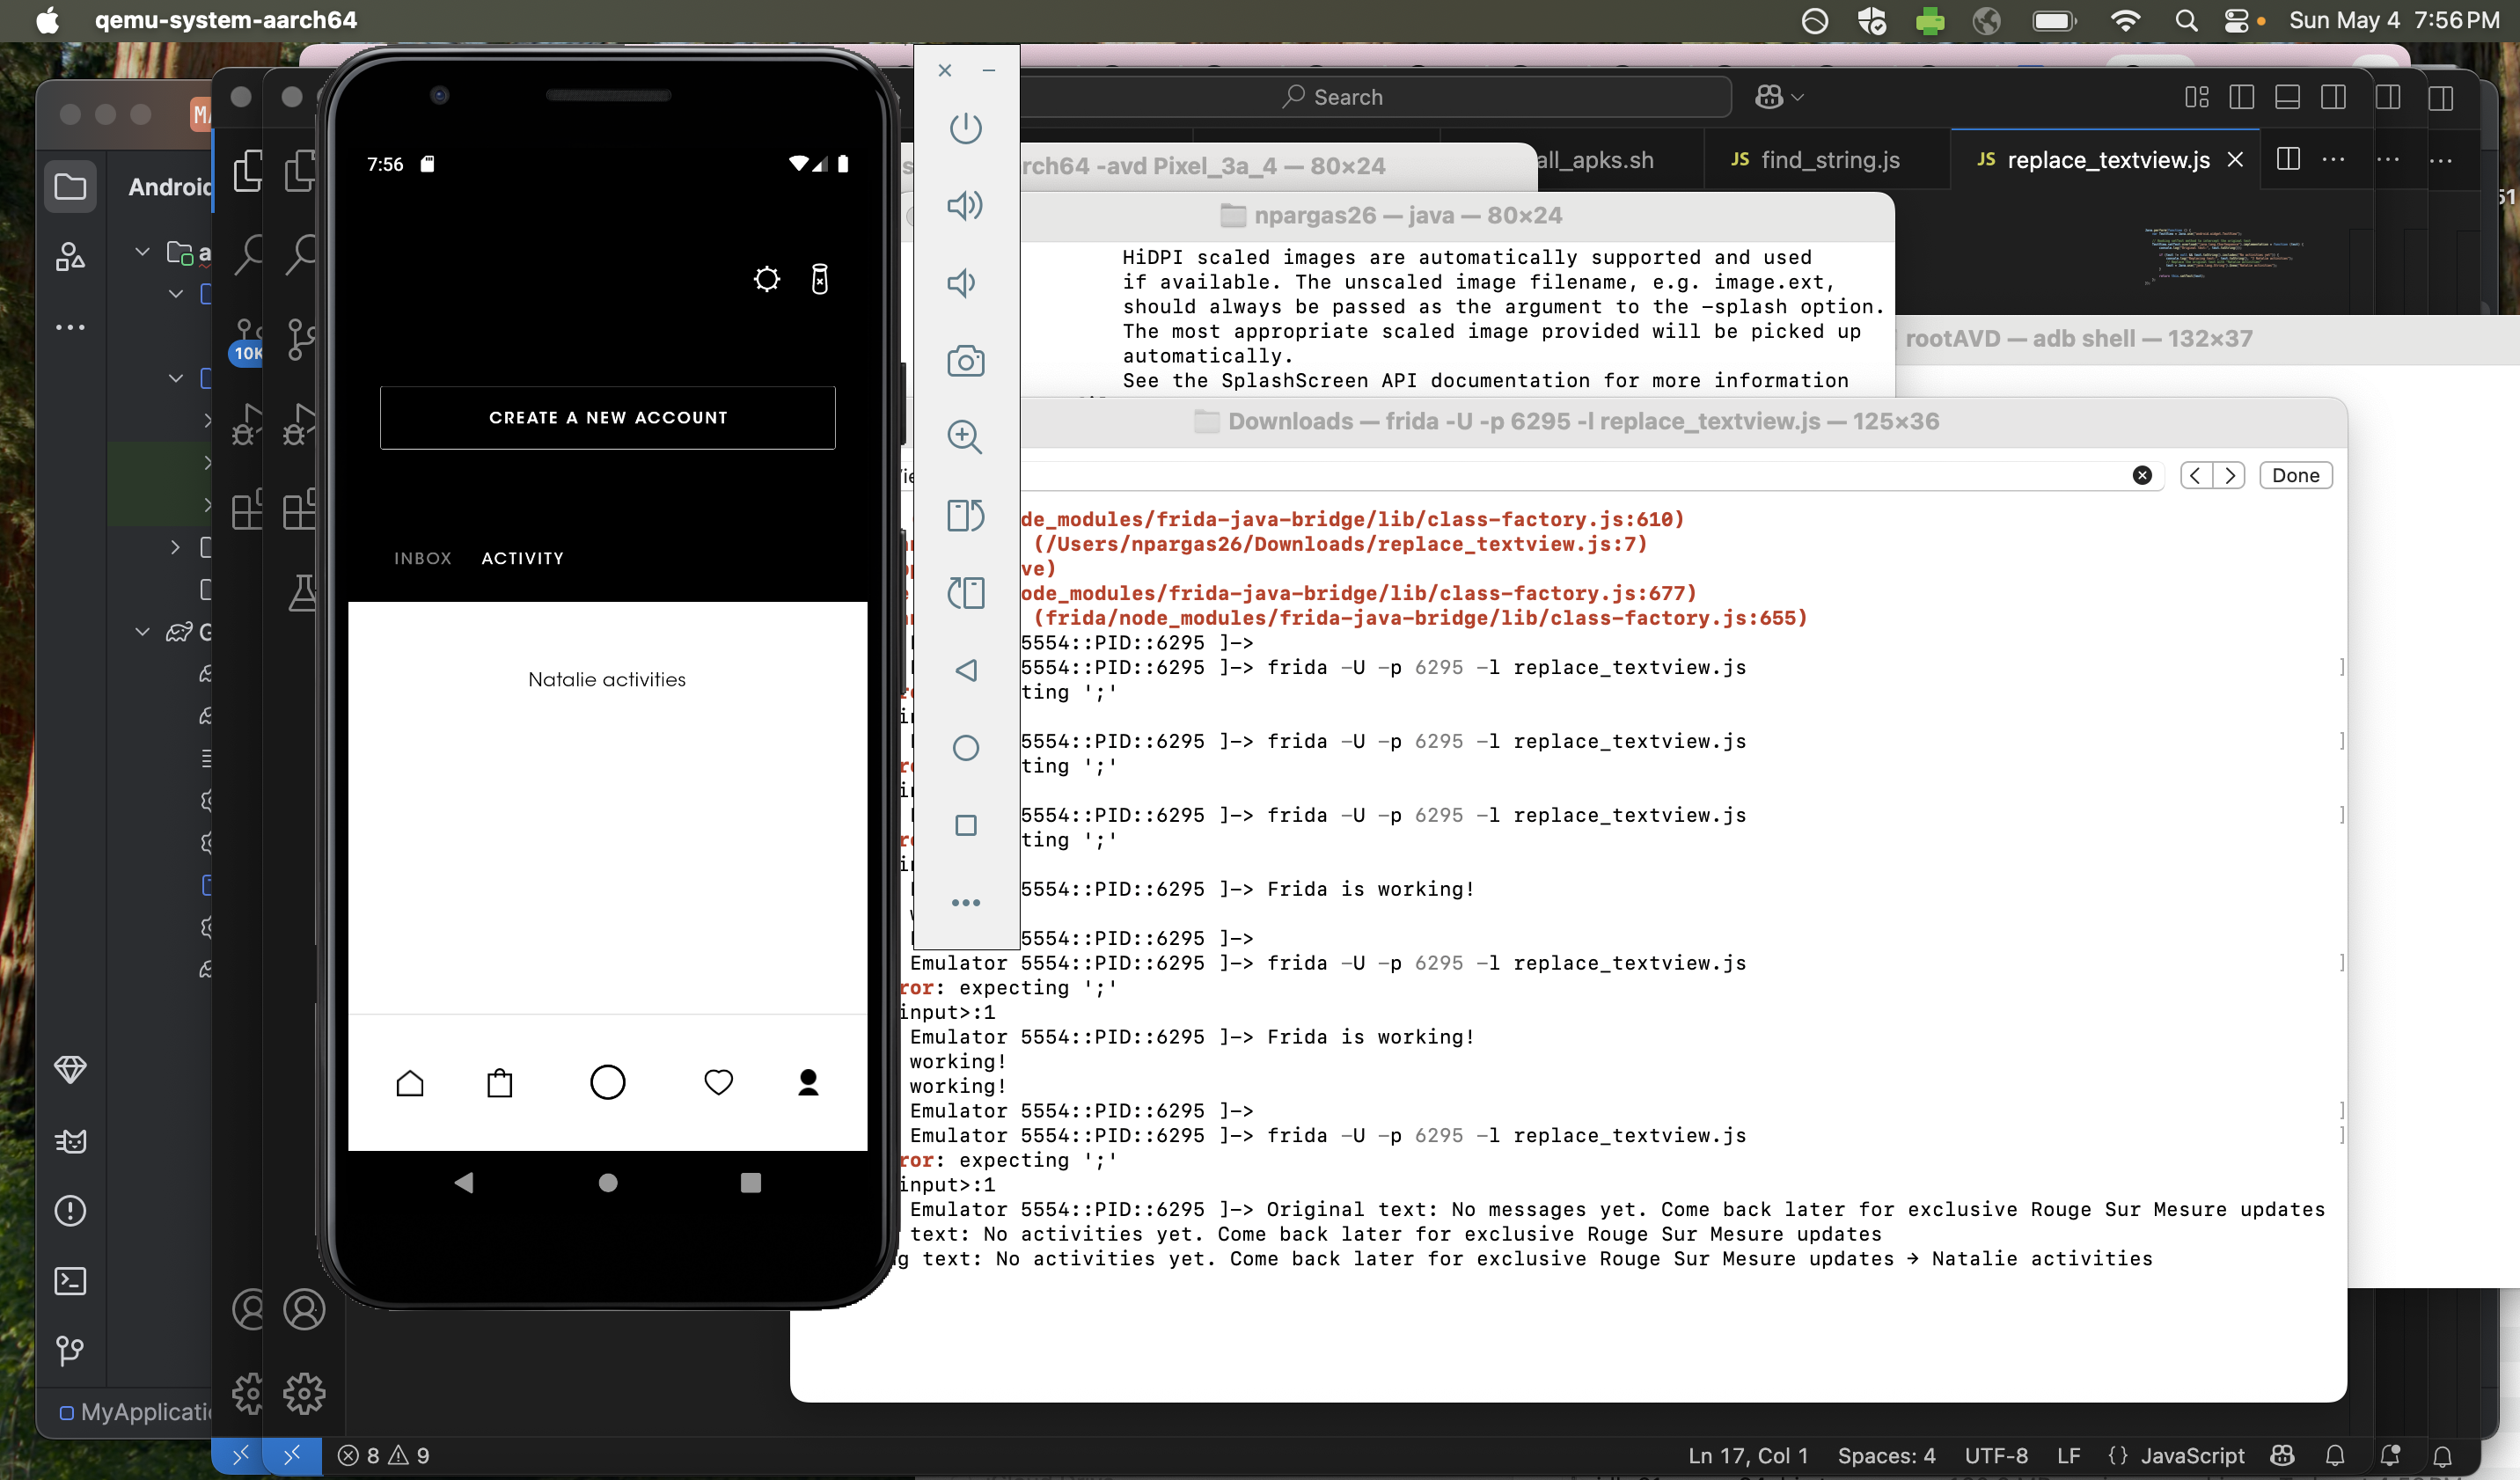
\includegraphics[scale=.15]{Natalie_activities}
	\caption{Altered App Screen}
	\label{fig:natalieactivities}
\end{figure}
